% ### Uses XeLaTeX ### %
% ### Needs beamer-master ### %
\documentclass[aspectratio=169]{beamer} %. Aspect Ratio 16:9
\usepackage{textgreek}
\usetheme{AI2} % beamerthemeSprace.sty
% DATA FOR FOOTER
\date{2019}
\title{}
\author{}
\institute{Advanced Institute for Artificial Intelligence (AI2)}
\begin{document}    
% ####################################
% FIRST SLIDE 						:: \SliTit{<Title of the Talk>}{<Author Name>}{<Intitution>}
% SLIDE SUB-TITLE					:: \SliSubTit{<Title of the Chapter>}{<Title of the Section>}
% SLIDE WITH TITLE 					:: \SliT{<Title>}{Content}
% SLIDE NO TITLE 						:: \Sli{<Content>} 
% SLIDE DOUBLE COLUMN WITH TITLE 	:: \SliDT{<Title>}{<First Column>}{<Second Column>}
% SLIDE DOUBLE COLUMN NO TITLE 		:: \SliD{<First Column>}{<Second Column>}
% SLIDE ADVANCED WITH TITLE 			:: \SliAdvT{<Title>}{<Content>}
% SLIDE ADVANCED  NO TITLE 			:: \SliAdv{<Content>}
% SLIDE ADVANCED DOUBLE TITLE 		:: SliAdvDT{<Title>}{<First Column>}{<Second Column>}
% SLIDE ADVANCED DOUBLE NO TITLE 	:: SliAdvD{<First Column>}{<Second Column>}
% ITEMIZE 							:: \begin{itemize}  \IteOne{1st Level} \IteTwo {2nd Level} \IteThr{3rd Level} \end{itemize}
% SECTION 							:: \secx{Section} | \secxx{Sub-Section}
% COLOR BOX 						:: \blu{blue} + \red{red} + \yel{yellow} + \gre{green}
% FRAME 							:: \fra{sprace} \frab{blue} \frar{red} + \fray{yellow} + \frag{green}	
% REFERENCE						:: \refer{<doi number>}
% FIGURE 							::  \img{X}{Y}{<scale>}{Figures/.png} 
% FIGURE							:: \begin{center}\includegraphics[scale=<#>]{Figures/.png}\end{center}
% PROJECT STATUS					:: \planned\~    \started\~   \underway\~   \done\~   
% EXERCICIO							:: \Exe{<#>}{<text>}
% STACKREL							:: \underset{<down>}{<up>}
% FLUSH LEFT						:: \begin{flalign*}  & <1st equation> & \\  & <12nd equation>  & \\ \end{flalign*}
% REAL / IMAGINAY					:: \Re / \Im
% SLASH								:: \sl{} or \sl
% BOLD MATH							:: \pmb{<>}
% ####################################
%
% FIRST SLIDE :: DO NOT BREAK LINE !!!
\SliTit{Probabilidades}{Advanced Institute for Artificial Intelligence}{https://advancedinstitute.ai}

\SliT{Probabilidades}{

Agenda

\begin{itemize}
\IteOne{Matplotlib}
\IteOne{Introdução a Probabilidade}
\IteOne{Distribuição de Probabilidade}
\IteOne{Exemplos de Distribuição de Probabilidade}
\IteOne{Teste de Hipótese}
\end{itemize}

}

\SliDT{Probabilidades}
{
\begin{itemize}
\IteOne{Matplotlib: biblioteca para criar gráficos}
\IteOne{Áreas do Gráfico controladas pela biblioteca}
\end{itemize}
}
{\begin{center}
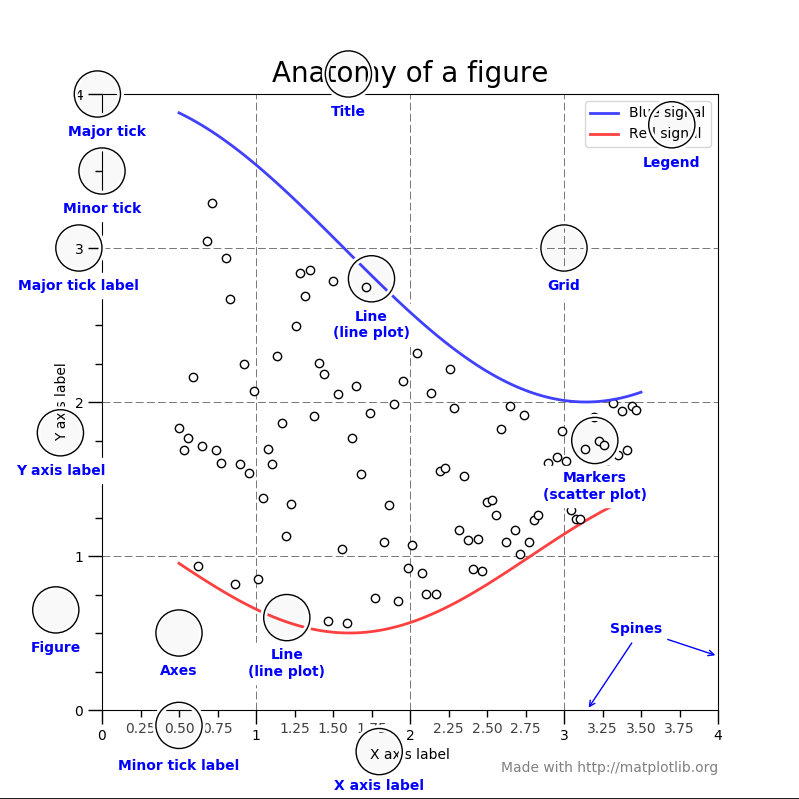
\includegraphics[scale=0.25]{11.png}     
\end{center}
}

\SliT{Probabilidades}
{
\begin{itemize}
\IteOne{Objeto pyplot: objeto da matplotlib}
\IteTwo{Cria figuras}
\IteTwo{Cria áreas em uma figura (Axes)}
\IteTwo{inclui diversos elementos ao gráfico: título, legenda, distribuições}
\end{itemize}
}

\SliT{Probabilidades}{

Probabilidade
\begin{itemize}

\IteOne{Pode ser usada como uma maneira de quantificar a incerteza associada a eventos escolhidos em um universo de eventos}
\IteTwo{Exemplo: rolar um dado}
\IteOne{O universo consiste em todos os resultados possíveis. 
qualquer subconjunto desses resultados é um evento}
\IteTwo{Dado: universo números de 1 a 6}
\IteTwo{exemplo de evento: dado retorna 1, dado retorna número maior que 3, jogando 10 vezes, sempre retorna um número maior que 2}

\end{itemize}
}

\SliT{Probabilidades}{

Eventos

\begin{itemize}
\IteOne{ P(E) probabilidade do evento E }
\IteOne{Quando analisamos probabilidade de dois ou mais evento, consideramos que tais ventos podem ser independentes ou dependentes}
\IteOne{Eventos independentes}
\IteTwo{dois eventos E e F são independentes se a probabilidade de
ambos acontecem é o produto das probabilidades de que cada um acontece}
\IteTwo{P(E,F) = P(E)*P(F))}
\IteOne{Eventos dependentes}
\IteTwo{P(E$|$F) = P(E,F)/P(F) probabilidade do evento E ocorrer caso F ocorra}

\end{itemize}

}

\SliT{Probabilidades}{

Nascimento de duas crianças (pode ocorrer menino ou menina)

\begin{table}[]
\begin{tabular}{lllll}
 & G & G  \\
 & B & B \\
 & G & B  \\
 & B & G  
\end{tabular}
\end{table}

\begin{itemize}
\IteOne{Probabilidade da mais velha ser meninas: $2/4$}
\IteOne{Probabilidade de duas meninas: $1/4$}
\IteOne{Probabilidade de uma das duas ser menina: $3/4$}
\end{itemize}
}

\SliT{Probabilidades}{

Variáveis Aleatórias

\begin{itemize}
\IteOne{Para uma variável (Contínua ou Discreta), uma distribuição de probabilidades determina as propriedades de cada evento }
\IteOne{A soma de todas as probabilidades de todos os eventos possíveis deve ser igual a 1 }
\IteOne{Se repetirmos um experimento com uma distribuição de probabilidade associada várias vezes, a probabilidade encontrada seguirá a distribuição de de uma variável aleatória }

\IteOne{Essa distribuição serve então como modelo padrão para uma população }

\end{itemize}

}

%\IteOne{O valor esperado $E(X)$ de uma variável aleatória, é a média de seus valores ponderados por suas probabilidades.}

\SliT{Probabilidades}{

A distribuição de probabilidade pode ser representada também usando fórmulas


\begin{itemize}
\IteOne{Função de densidade de probabilidade (PDF)}
\IteTwo{Para cada valor a função retorna uma probabilidade associada a esse valor}
\IteOne{Função de distribuição acumulada}
\IteTwo{Descreve como probabilidades são associadas a intervalos de valores de uma variável aleatória.}
\IteTwo{Calculada como a integral da função de densidade de probabilidade}
\end{itemize}

}

\SliT{Probabilidades}{

\begin{itemize}
\IteOne{Diversos tipos de Distribuições de probabilidades possuem possuem características adequadas para modelar fenômenos específicos}
\IteTwo{Binomial: distribuições binárias, probabilidade de algo ocorrer ou não ocorrer}
\IteTwo{Uniforme: eventos possuem probabilidades estatisticamente muito próximas}
\IteTwo{Poisson: modela número de eventos que podem ocorrer em um período de tempo ou área }

\end{itemize}

}

\SliT{Probabilidades}{

\begin{itemize}
\IteOne{As distribuições conhecidas e formalizadas possuem fórmulas para gerar a distribuição de probabilidade}
\IteOne{As bibliotecas numpy e scipy por exemplo, permitem gerar tais distribuições com base em parâmetros iniciais}
\IteOne{Tais funções permitem reproduzir fenômenos ou recriar cenários quando a distribuição de probabilidades é conhecida}
\end{itemize}

}

\SliT{Probabilidades}{

\begin{itemize}
\IteOne{Distribuição Uniforme}
\IteOne{Uma variável aleatória X que distribuição Uniforme no intervalo [a, b] }
\IteOne{PDF da função abaixo }
\IteOne{CDF da função abaixo: é a probabilidade acumulativa }
\IteTwo{probabilidade de dar um valor próximo de b é maior do que entre valor no meio do intervalo [a , b], pois a área é maior}

\end{itemize}

\begin{center}
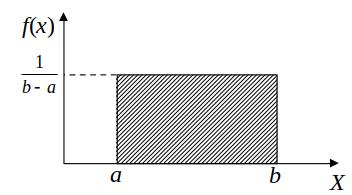
\includegraphics[scale=0.45]{12.png}     
\end{center}
}

%\SliT{Probabilidades}{
%\begin{itemize}
%\IteOne{Distribuição de Bernoulli}
%\IteOne{Considere uma variável X que apresenta apenas 2 valores possíveis, 0 e 1, sendo que P(X = 1) = p e P(X = 0) = 1 – p. Geralmente, associa-se o valor 1 ao sucesso e 0 ao fracasso, sendo assim, p é a probabilidade de sucesso e q de fracasso.}
%\end{itemize}

%\begin{center}
%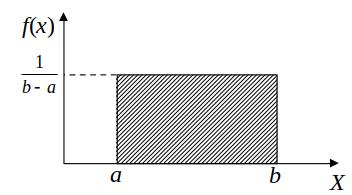
\includegraphics[scale=0.45]{12.png}     
%\end{center}
%}

\SliT{Probabilidades}{

Teste de Hipótese

\begin{itemize}
\IteOne{Hipótese é uma assertiva que podemos provar ou refutar}
\IteOne{Refutar normalmente leva a um avanço do conhecimento}
\IteOne{Em estatística tenta-se por padrão provar que uma assertiva está errada, para concluir alguma coisa a partir de levantamento estatísticos}
\end{itemize}

}

\SliT{Probabilidades}{

Teste de Hipótese

\begin{itemize}
\IteOne{Hipótese estatística: suposição quanto ao valor de um parâmetro populacional, ou quanto à natureza da distribuição de probabilidade de uma variável populacional.}
\IteOne{teste de Hipótese: É uma regra de decisão para aceitar ou rejeitar uma hipótese estatística com base nos elementos amostrais}
\end{itemize}

}

\SliT{Probabilidades}{

Tipos de Hipótese

\begin{itemize}
\IteOne{hipótese nula H0 é hipótese estatística a ser testada}
\IteOne{H 1 é a hipótese alternativa.}
\IteOne{H0 é uma assertiva de como a realidade deveria ser, se nossa suposição estivesse errada}
\IteOne{A hipótese nula expressa uma igualdade}
\IteOne{hipótese alternativa é dada por uma desigualdade}
\end{itemize}

}

\SliT{Probabilidades}{

\begin{itemize}
\IteOne{O teste de hipótese retorna um valor de significância chamado P-valor (\textit{P-value})}
\IteOne{O P-valor é definido como a probabilidade de obter um resultado igual ou mais extremo do que realmente foi observado.}
\IteOne{Quanto menor o p-valor, maior a significância, pois indica a investigador de que a hipótese em consideração pode não expliquar adequadamente a observação.}

\IteOne{P-valor representa o critério para rejeitar ou não-rejeitar a hipótese nula}
\IteOne{Um valor padrão para P-valor é 0.05}

\end{itemize}


}

%\SliT{Probabilidades}{

%Intervalo de confiança

%\begin{itemize}
%\IteOne{}
%\end{itemize}

%}

%\SliT{Estatística}{

%Separar dados em Treino e Teste

%\begin{itemize}
%\IteOne{test\_size}
%\IteOne{train\_size}
%\IteOne{random\_state}
%\IteOne{shuffle}

%\end{itemize}

%}

\end{document}